%% Small qualitative ablation figure (one column). Graphic: figures/ablation_qualitative.png
%% 5 columns x 4 rows. Columns, left to right:
%%   ours w/o refinement (the coarse transfer) | ours w/o temporal FiLM |
%%   ours w/o normal concatenation | ours (full) | ground truth
%% Rows are four different query touch locations. Column headers are baked into the image.
\begin{figure}[t]
  \centering
  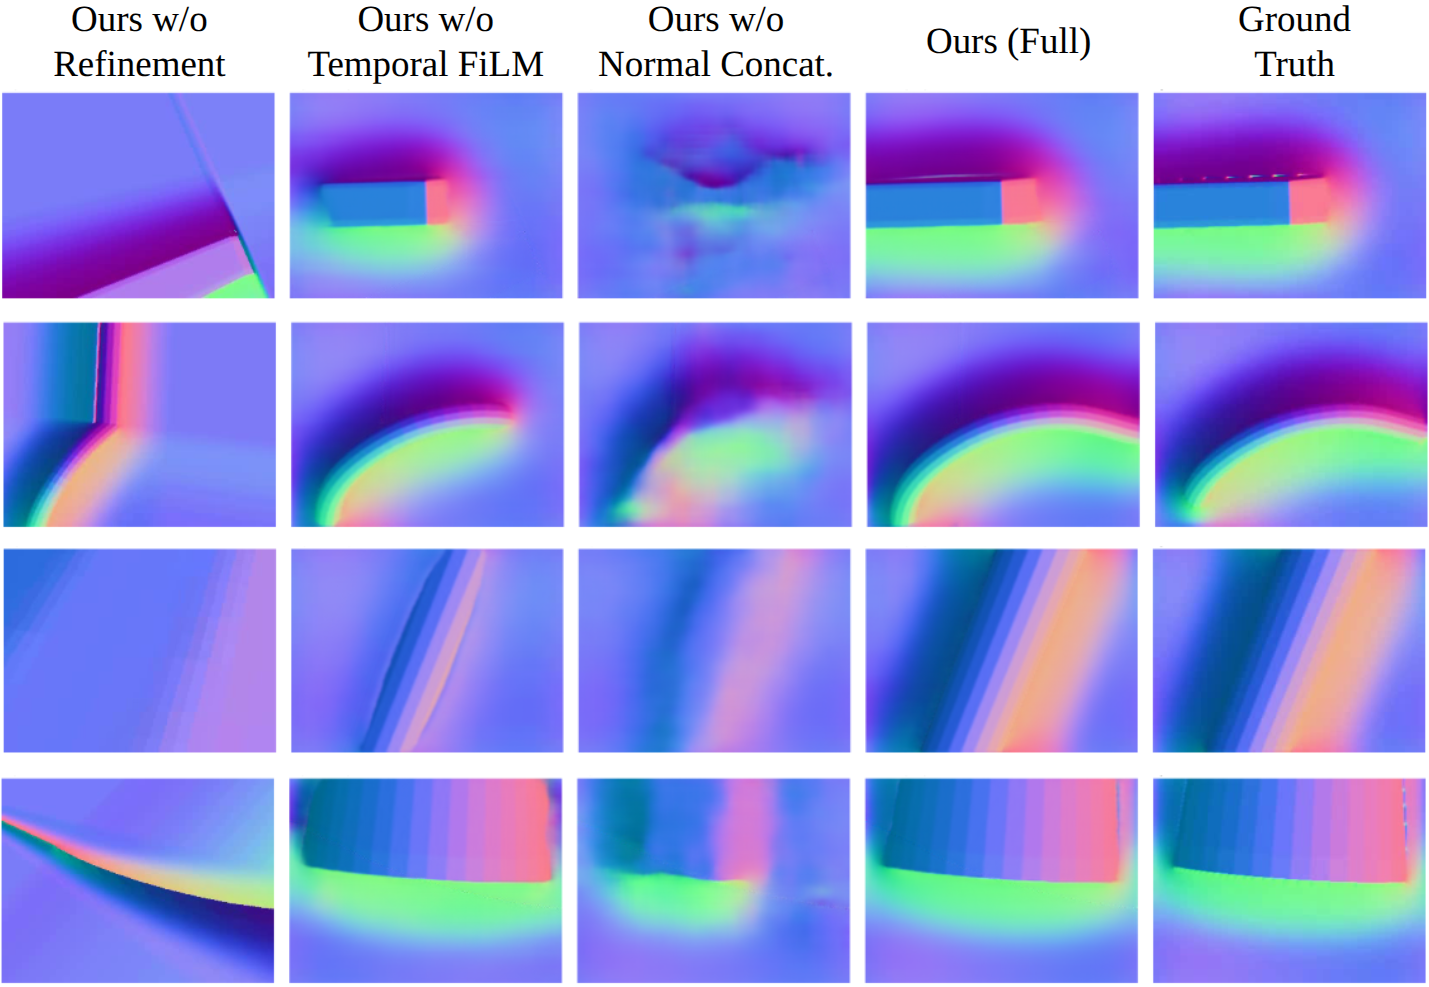
\includegraphics[width=\linewidth]{figures/ablation_qualitative.png}
  \caption{\textbf{Qualitative ablation of the refinement stage.} Each row is one query touch
    location, shown at the deepest-contact frame. From left to right: the coarse transfer with no
    neural refinement, refinement without temporal conditioning through FiLM, refinement without
    the concatenated query normal map, our full model, and the ground truth. Removing either
    conditioning signal degrades the prediction in a characteristic way. Without the query normal
    map the network has no evidence about the surface it is predicting for, and its output loses
    the contact geometry almost entirely. Without the timestamp the network cannot tell how deep
    into the press it is, so it recovers the shape of the contact but softens the edges that the
    full model keeps sharp.}
  \label{fig:ablation}
\end{figure}
